%%本章讲解关于svm,\phontom{}中为占位符.
\documentclass[UTF8]{ctexart}
\usepackage{geometry}
\usepackage{graphicx}
\usepackage{latexsym,bm,amsmath,amssymb}
\geometry{a4paper,scale=0.8}
\title{Support Vector Machine}
\author{AsukaShiKi}
\date{\today}
\begin{document}
\maketitle
\par
\begin{figure}[ht]
    \centering
    
\includegraphics[scale=0.15]{01.jpg}
\end{figure}
\begin{figure}[ht]
    \centering
    
\includegraphics[scale=0.5]{02.jpg}
\end{figure}
\newpage
\tableofcontents
\newpage
\large{
\section{支持向量机}
支持向量机(Support Vector Machine,简称SVM)是一种针对二分类任务设计的分类器,它的理论相对神经网络模型来说更加完
备和严密,并且效果显著,结果可预测,是非常值得学习的模型。\\
本章内容包括有:\par
间隔与支持向量:如何计算空间中任一点到超平面的距离?什么是间隔?什么是支持向量?支持向量机求解的目标是什么?\par
对偶问题:求取最大间隔等价于怎样的对偶问题?KKT条件揭示出支持向量机的的什么性质?如何用SMO算法快速求解?为什么SMO算
法可以快速求解?\par
核函数:如何处理非线性问题?什么是核函数?为什么需要核函数?有哪些常用的核函数?核函数具有什么性质?\par
软间隔和正则化:如何应对过拟合问题?软间隔和硬间隔分别指什么?如何求解软间隔支持向量机?0/1损失函数具有哪些可选的损失
替代函数?\par
支持向量回归:什么是支持向量回归?与传统回归模型有什么不同?支持向量回归的支持向量满足什么条件?\par
核方法:什么是核方法?什么是表示定理?如何应用?\newpage

\section{间隔与支持向量}
\subsection{点到超平面的距离}
设\bm{$\omega$$^T$}x+b=0是超平面的表达式,则超平面的法向量是\bm{$\omega$},证明如下:任取超平面上两点x$_1$,x$_2$,
则两点均满足超平面方程,且两点连线x$_1$x$_2$所在直线也在超平面上,两点连线的向量形式则为两点向量差x$_1$-x$_2$,则有
\bm{$\omega$$^T$}(x$_1$-x$_2$)=\bm{$\omega$$^T$}x$_1$+b-(\bm{$\omega$$^T$}x$_2$+b)=0-0=0;所以得证\bm{$\omega$}
垂直于$\overrightarrow{x_1x_2}$,即\bm{$\omega$}是超平面\bm{$\omega$$^T$}x+b=0的法向量。\par

设有超平面\bm{$\omega$$^T$}x+b=0,空间中一点x,超平面上一点y,则点x到超平面的距离即为向量$\overrightarrow{xy}$在
超平面法向量\bm{$\omega$}方向上的投影长度。则点x到超平面距离:\par

\begin{center}
    {\Large dist\footnote{$||\bm{\omega}||$是$\omega$的欧几里得范数}
                 = $\frac{|\bm{\omega^T}\overrightarrow{xy}|}{||\bm{\omega}||}$
                 = $\frac{|\bm{\omega^T}{(x-y)}|}{||\bm{\omega}||}$
                 = $\frac{|\bm{\omega^T}x-\bm{\omega^T}y|}{||\bm{\omega}||}$
                 = $\frac{|\bm{\omega^T}x-(0-b)|}{||\bm{\omega}||}$}
\end{center}
即有:
\begin{center}
    {\Large dist = $\frac{|\bm{\omega^T}x+b|}{||\bm{\omega}||}$}
\end{center}

由上述推导可知,超平面外任一点x到超平面\bm{$\omega$$^T$}x+b=0的距离都是$\frac{|\bm{\omega^T}x+b|}{||\bm{\omega}||}$。
\subsection{支持向量}
给定一个二分类数据集,正类标记标记为+1,负类标记为-1;分类学习试图从样本空间找到一个超平面,使得超平面可以将不同类
的样本分开。满足要求的超平面可能会有很多,我们需要找到最优的超平面。\par
在svm中,我们试图找到处于两类样本正中间的超平面,这样的超平面对于训练数据局部扰动的容忍性最好,新样本也不容易被误分
类;也就是这样的超平面对未见示例的泛化能力最强(如图1)。\par
图一中实线即为划分超平面,在线性模型中可以通过方程\bm{$\omega$$^T$}x+b=0来表示,在二维样本空间中就是一条直线。\bm
{$\omega$}是线性模型的权重向量(又叫投影向量),也是划分超平面的法向量,决定着超平面的方向。偏置项b又被称为位移项,
决定了超平面和空间原点之间的距离。\par
假设超平面可以将所有样本正确分类,即对于样本点(x,y)有标记y=+1的点有\bm{$\omega$$^T$}x+b\\>0,对所有标记y=-1的点有
\bm{$\omega$$^T$}x+b<0。

\begin{figure}[ht]
    \centering
    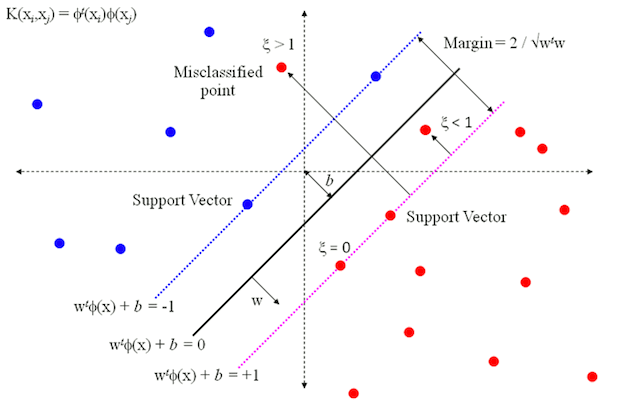
\includegraphics[scale=0.7]{71187447_p0.png}
    \caption{对样本空间分类的超平面示例图}
\end{figure}
只要存在这样一个超平面,那么我们就可以对参数\bm{$\omega$}和b进行适当的放缩,使得有:
\begin{center}
    {\Large \bm{$\omega$$^T$}x + b $\geq$ +1,y = +1\\[3ex]
            \bm{$\omega$$^T$}x + b $\leq$ -1;y = -1
    }
\end{center}\par
而SVM中使得上式等号成立的训练样本点就是支持向量(Support Vector),它们是距离超平面最近的几个样本点,也即上面图中两
条虚线上的点(图中存在比支持向量距离超平面更近的点,这跟软间隔有关,这里先不讨论)。在SVM中,我们希望实现的是最大化
两类支持向量到超平面的距离之和,那首先就得知道怎么计算距离。怎样计算样本空间中任意数据点到划分超平面的距离我们在上
一节中已经讲过。
\subsection{间隔}
如2.2节所述,我们想要实现的是最大化两类支持向量到超平面的距离之和,如图一所示,根据定义我们有:
\begin{center}
    {
        \Large
        { 
            \bm{$\omega$$^T$}x + b = +1;y = +1\\[3ex]
            \bm{$\omega$$^T$}x + b = -1;y = -1
        }
    }
\end{center}
带入2.1节的距离公式可得支持向量到超平面的距离是$\frac{1}{\bm||\bm{\omega}||}$。\par
我们定义\textbf{间隔(margin)}为两个异类支持向量到超平面的距离之和为:\par
\begin{center}
    \Large \bm{$\gamma$} = 2 * $\frac{1}{\bm||\bm{\omega}||}$ = $\frac{2}{\bm||\bm{\omega}||}$\\[2ex]
\end{center}
SVM的目标就是找到具有最大间隔的划分超平面,也即找到是\bm{$\gamma$}最大的参数\bm{$\omega$}和b进行适当的放缩,使得
有:\par
\begin{center}
    \Large{
        $\max\limits_{\omega,b}$$\frac{2}{||\bm{\omega}||}$\\[1ex]
        $\quad s.t.\quad y_i(\omega^Tx+b)\geq1,i=1,2,3,......m$
        }
\end{center}
约束部分指的是全部样本都被正确分类,此时标记值(+1或−1)乘上预测值(≥+1或≤−1)必定是一个≥1的数值。看上去间隔大小
只与$\omega$有关,但实际上位移项b也通过约束影响着$\omega$的取值,进而对间隔产生影响。由于最大化$||\bm{\omega}||^{-1}$
等价于最小化$||\bm{\omega}||^2$,所以可以重写目标函数为:\par
\begin{center}
    \Large{
        $\min\limits_{\omega,b}$$\frac{||\bm{\omega}||^2}{2}$\\[2ex]
        $\quad s.t.\quad y_i(\omega^Tx+b)\geq1,i=1,2,3,......m$(1)
    }
\end{center} 
我们引入$\frac{1}{2}$的原因是为了求导时可以约去平方项的2,式(1)就是支持向量机的基本型。特别地,我们还有以下定义:\par
\begin{center}
    函数间隔:$y_i(\omega^Tx+b)$\\[3ex]
    几何间隔:\Large{
        $\frac{y_i(\omega^Tx+b)}{||\bm{\omega}||^2}$
    }
\end{center}\newpage
\section{对偶问题}
\subsection{拉格朗日乘子}
式(1)是一个带约束的凸二次规划问题(凸问题意味一定有全局最优解,而不会陷入局部最优解)。本节介绍使用拉格朗日乘子计算最
优解的方法。\par
拉格朗日乘子方法的过程大致可以分为以下几步,对于待求目标:$min_xf(x),s.t.h(x)=0,g(x)\leq0$:\par
(a).拉格朗日函数$L(x,\lambda,\mu)=f(x)+\lambda h(x)+\mu g(x)$\par
(b).令$\frac{\partial L(x,\lambda,\mu)}{\partial x}=0$,解出用$\lambda$,$\mu$表示出的$x$\par
(c).将$x$带入$L(x,\lambda,\mu)$中得:$\Gamma(\lambda,\mu)=min_xL(x,\lambda,\mu)$\par
(d).对偶问题即为:$max_{\lambda,\mu}\Gamma(\lambda,\mu),s.t.\mu\geq0$\par
\subsection{应用拉格朗日乘子到式(1)}
回到式(1)\begin{center}
    \Large{
        $\min\limits_{\omega,b}$$\frac{||\omega||^2}{2}$\\[2ex]
        $\quad s.t.\quad y_i(\omega^Tx+b)\geq1,i=1,2,3,......m$(1)
    }
\end{center}\par
为式(1)的每个约束条件添加拉格朗日乘子$a_i\geq0$(对应m个样本的m个约束),得到该问题的拉格朗日函数:
\begin{center}
    \Large{
        $L(\omega,b,a)=\frac{1}{2}||\omega||^2+\sum\limits_{i=0}\limits^m$$a_i(1-y_i(\omega^Tx_i+b))$\quad(2)
    }
\end{center}\par
其中$a=(a_1,a_2,a_3,......,a_m)$,对拉格朗日函数求关于$\omega,b$的偏导数,并令偏导为零。\par
\begin{center}
    偏导数:\Large{
        $\frac{\partial L(\omega,b,a)}{\partial \omega}=\omega-\sum\limits_{i=1}\limits^ma_iy_ix_i$(3)\\[2ex]
        \phantom{偏导数:}$\frac{\partial L(\omega,b,a)}{\partial b}=-\sum\limits_{i=1}\limits^ma_iy_i\phantom{111}(4)$
    }
\end{center}\par
令式(3)(4)为0,得$\omega=\sum\limits_{i=1}\limits^ma_iy_ix_i$,$\sum\limits_{i=1}\limits^ma_iy_i=0$。\par
将式(3)带入式(1)消去$\omega$,再由约束条件式(4)消去b,得到式(1)的对偶问题(附推导过程):\par
\begin{center}
    \Large{
        $L(\omega,b,a)=\frac{1}{2}\omega^T\omega+\sum\limits_{i=0}\limits^ma_i-\sum\limits_{i=0}\limits^ma_iy_i\omega^Tx_i-\sum\limits_{i=0}\limits^ma_iy_ib$\\
        $\phantom{aaaaaaaaaaa}=\frac{1}{2}\omega^T\omega+\sum\limits_{i=0}\limits^ma_i-\omega^T(\sum\limits_{i=0}\limits^ma_iy_ix_i)-b(\sum\limits_{i=0}\limits^ma_iy_i)$\newpage
        $L(\omega,b,a)=\frac{1}{2}\omega^T\omega+\sum\limits_{i=0}\limits^ma_i-\omega^T\omega-0$\\
        $=\sum\limits_{i=0}\limits^ma_i-\frac{1}{2}\omega\omega^T\phantom{a}$ 
    }
\end{center}
将$\omega=\sum\limits_{i=1}\limits^ma_iy_ix_i$带入上式可得式(1)的对偶问题:\par
\begin{center}
    \Large{
        $\max\limits_a\sum\limits_{i=1}\limits^ma_i-\frac{1}{2}\sum\limits_{i=1}\limits^m\sum\limits_{j=1}\limits^ma_ia_jy_iy_jx_i^Tx_j$\\[2ex]
        $s.t.\sum\limits_{i=1}^ma_iy_i=0,a_i\geq0,i=1,2,3,....,m$\quad(5)
    }
\end{center}\par
解出$max$值$a_i$后,可以求出$\omega,b$得到模型:\par
\begin{center}
    \Large{
        $f(x)=\omega^Tx+b=\sum\limits_{i=1}^ma_iy_ix_i^Tx_i+b$\quad(6)
    }
\end{center}\par
我们在式(5)解出的$max$值$a_i$是式(2)的拉格朗日乘子,对应训练样本($x_i,y_i$),由于式(1)有不等式约束,
所以求解过程需要满足KKT条件:\par
$$ \left\{
\begin{aligned}
    a_i & \geq & 0 \\
    y_if(x_i)-1 & \geq & 0 \\
    a_i(y_if(x_i)-1) & = & 0
\end{aligned}
\right.
$$\par
这个KKT条件说明了,对任何一个样本$x_i$来说,要么对应的拉格朗日乘子$a_i$为0,此时样本$x_i$对式(6)毫无
贡献,不会影响到模型;要么函数间隔$y_if(x_i)=1$,此时样本$x_i$位于最大间隔边界上,是一个支持向量。它
揭示了SVM的一个重要性质:最终模型只与支持向量有关,因此训练完成后,大部分的训练样本都不需保留。
\subsection{$SMO$算法}
对偶问题式(5)是二次规划问题,为避免通用二次规划算法求解是问题规模正比于样本数的问题,我们使用高效的$SMO$
算法。\par
初始化参数$a$后,$SMO$算法重复下面两个步骤直至收敛:\par
\begin{center}
    1.选取一对需要更新的变量$a_i$和$a_j$。\phantom{更更更更更更更更更更aaaa}\\
    2.固定$a_i$和$a_j$之外的参数,求解对偶问题式(5)来更新$a_i$和$a_j$。
\end{center}\par
\subsubsection{\large{选取$a_i$和$a_j$}}
首先我们要知道,只要我们选取的$a_i$,$a_j$有一个不满足KKT条件,那么更新后的目标函数的值就会变大,而且违背
KKT条件的程度越大,更新后的目标函数值增幅越大。\newpage
由此,$SMO$算法先选取一个违背KKT条件程度最大的变量$a_i$,再选取一个使目标函数增长最快的变量$a_j$,但由于
找出$a_j$的开销较大,所以$SMO$算法采用了一个启发式算法,使选取的两变量对应的样本之间间隔最大,这样的两个
变量差别很大,与选取两个相似的变量相比,这种方法能为目标函数带来更大的变化,从而更快的搜索到全局最大值。\par
由于每次迭代中,$SMO$算法只选取两个参数,其他参数固定,所以效率较高。由此,可以将式(5)的约束重写为:\par
\begin{center}
    \Large{
        $a_iy_i+a_jy_j=c,a_i\geq0,a_j\geq0$\quad(7)
    }
\end{center}
其中,$c=-\sum_{k\neq i,j}a_ky_k$看作是固定的常数。
\subsubsection{\large{计算$\omega$和$b$}}
利用式(7),可以将$a_j$从式(5)中消去,考虑$a_i\geq 0$约束,可以直接算出$a_i,a_j$。使用SMO算法计算出最优解
之后,我们关注的是如何推出$\omega$和$b$ ,从而得到最终模型。获得$\omega$很简单,直接用式(3)=0就可以了。
而位移项$b$则可以通过支持向量导出,因为对于任一支持向量$(x_s,y_s)$,都有函数间隔等于1,所以有:\par
\begin{center}
    \Large{
        $y_sf(x)=y_s(\sum\limits_{i\in S}a_iy_ix_i^Tx_s+b)=1$\quad(8)
    }
\end{center}\par
这里的$S$是所有支持向量的下标集(事实上,用所有样本的下标也行,不过非支持向量的拉格朗日乘子等于0,对求和没
贡献,这一点前面已经提到了)。理论上,我们只要选取任意一个支持向量代入式(8)就可以把$b$算出来了。但实际任务
中往往采用一种更鲁棒的做法:用所有支持向量求解的平均值:
\begin{center}
    \Large{
        $b=\frac{1}{|S|}\sum\limits_{s\in S}(\frac{1}{y_s}-\sum\limits_{i\in S}a_iy_ix_i^Tx_s)$
        }
\end{center}\newpage
\section{核函数}
\subsection{处理非线性划分}
在现实任务中,我们更常遇到的是在原始样本空间中非线性可分的问题。对这样的问题,一种常用的思路是将样本从原始
空间映射到一个更高维的特征空间,使得样本在该特征空间中线性可分。幸运的是,只要原始空间是有限维的(也即属性
数目有限),那就必然存在一个高维特征空间使样本线性可分,举例如下,二维平面上若干样本点呈如下分布:\\[2ex]
\begin{figure}[ht]
    \centering
    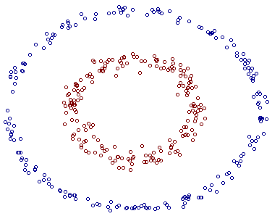
\includegraphics[scale=1.0]{02.png}
    \caption{二维平面样本点分布图}
\end{figure}\par
此时划分两类样本,需要一个非线性的圆形曲线,假设原始空间中两个属性分别是$x,y$,如果我们做一个映射,把样本点
都映射到一个三维特征空间,维度取值分别为$x^2,y^2,y$,则得到下面的分布:\\[2ex]
\begin{figure}[ht]
    \centering
    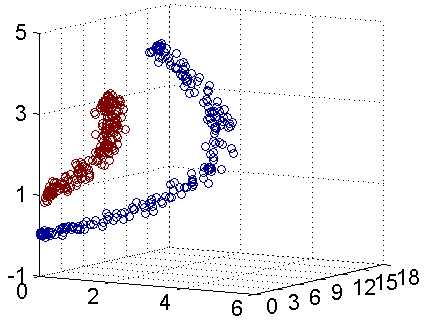
\includegraphics[scale=0.7]{03.png}
    \caption{三维映射图}
\end{figure}\par
映射过后,可以看见我们只需要一个线性超平面就可以将两类样本点分开。
\subsection{核函数定义}
在上一节例子中,我们将每个样本对应的二维特征向量x映射为一个三维的特征向量,假设我们用$\phi(x)$来表示映射所得
特征向量。则在映射的高维特征空间中,用于划分的线性超平面可以表示为:
\begin{center}
    \Large{
        $f(x)=\omega^T\phi(x)+b$
    }
\end{center}\par
类似式(1),可以得到此时的目标函数为:
\begin{center}
    \Large{
        $\min\limits_{\omega,b}\frac{1}{2}||\omega||^2$\quad(9)\\[2ex]
        $s.t.\quad y_i(\omega^T\phi(x)+b)\geq1,i=1,2,3,....,m$
    }
\end{center}\par
对应的对偶问题为:
\begin{center}
    \Large{
        $\max\limits_{a}\sum\limits_{i=1}\limits^ma_i-\frac{1}{2}\sum\limits_{i=1}\limits^m\sum\limits_{j=1}
        \limits^ma_ia_jy_iy_j\phi(x_i)^T\phi(x_j)$\quad(10)\\[2ex]
        $s.t.\quad\sum\limits_{i=1}\limits^ma_iy_i=0,a_i\geq 0,i=1,2,....,m$
    }    
\end{center}
式(10)中的$\phi(x_i)^T\phi(x_i=j)$是向量$x_i,x_j$映射到高维空间后的内积,由于特征空间维数可能会很高,所以直接计算映
射后的特征向量的内积很困难,如果映射后的特征空间是无限维的,则根本无法计算。\par
为了解决这样的问题,引入了核函数;假设输入空间是二维的,每个样本点有两个属性$x,y$,存在映射将每个样本点映射到三维空间:
\begin{center}
    \Large{
        $\phi(x)=\phi(x,y)=(x^2,\sqrt{2}xy,y^2)$
    }
\end{center}\par
给定原始空间中的两个样本点$V_1=(x_1,y_1)$和$V_2=(x_2,y_2)$,则他们映射到高维特征空间后的内积可以写作:
\begin{align*}
        \phi(V_1)^T\phi(V_2)&=<\phi(V_1),\phi(V_2)>\\
        &=<(x_1^2,\sqrt{2}x_1y_1,y_1^2),(x_2^2,\sqrt{2}x_2y_2,y_2^2)>\\
        &=x_1^2x_2^2+2x_1x_2y_1y_2+y_1^2y_2^2\\
        &=(x_1x_2+y_1y_2)^2\\
        &=<V_1,V_2>^2\\
        &=\kappa(V_1,V_2)
\end{align*}
从上面的例子中可以看出高维特征空间中两个点的内积,可以写成一个关于原始空间中两个点的函数$\kappa(,;,)$,这个就是核函数,
上面的例子用的就是多项式核,多项式次数$d$取2。
\subsection{为何需要核函数}
这里的例子为了计算方便,映射的空间维数依然很低,所以稍微解释一下为什么需要核函数?假设原始空间是二维的,那么对于两个属
性$x$和$y$,取一阶二阶的组合只有5个(即$x^2,y^2,x,y,xy$)。但当原始空间是三维的时候,仍然取一阶二阶,组合就多达19个了
($x,y,z,xy,xz,yz,xyz,x^2y,x^2z,y^2x,y^2z,z^2x,z^2y,x^2yz,xy^2z,xyz^2,x^2y^2z,x^2yz^2,xy^2z^2$)。随着原始空间
维数增长,新空间的维数是呈爆炸性上升的。何况现实中我们遇到的问题的原始空间往往本来就已经是高维的,如果再进行映射,新
特征空间的维度是难以想象的。\par
然而有了核函数,我们就可以在原始空间中通过函数$\kappa(.;.)$计算(这称为核技巧(kernel trick)),而不必直接计算高维甚至
无穷维特征空间中的内积。\par
使用核函数后,对偶问题式(10)可以重写为:
\begin{center}
    \Large{
        $\max\limits_a\sum\limits_{i=1}\limits^ma_i-\frac{1}{2}\sum\limits_{i=1}\limits^m\sum\limits_{j=1}\limits^m
        a_ia_jy_iy_j\kappa(x_i;x_j)$\\
        $s.t. \sum\limits_{i=1}\limits^ma_iy_i=0,a_i\geq0,i=1,2,3,....,m$\quad(11)
    }
\end{center}
求解后得到的模型可以表示为:
\begin{align*}
    f(x) &=\omega^T\phi(x)+b\\
         &=\sum\limits_{i=1}\limits^ma_iy_i\phi(x_i)^T\phi(x)+b\\
         &=\sum\limits_{i=1}\limits^ma_iy_i\kappa(x_i;x)+b
\end{align*}\\
这条式子表明了模型最优解可通过训练样本的核函数展开,称为支持向量展式(support vector expansion)。在需要对新样本进行
预测时,我们无需把新样本映射到高维(甚至无限维)空间,而是可以利用保存下来的训练样本(支持向量)和核函数$\kappa$进行求
解。\\
注意,核函数本身不等于映射;它只是一个与计算两个数据点映射到高维空间之后的内积等价的函数。当我们发现数据在原始空间线性
不可分时,会有把数据映射到高维空间来实现线性可分的想法,比方说引入原有属性的幂或者原有属性之间的乘积作为新的维度。假
设我们把数据点都映射到了一个维数很高甚至无穷维的特征空间,而模型求解和预测的过程需要用到映射后两个数据点的内积,这时
直接计算就没辙了。但我们又幸运地发现,原来高维空间中两点的内积在数值上等于原始空间通过某个核函数算出的函数值,无需先
映射再求值,就很好地解决了计算的问题了。
\subsubsection{核函数的性质}
核函数定理:给定一个输入空间$\chi$,函数$\kappa(.;.)$是定义在$\chi\times\chi$上的对称函数。当且仅当对于任意数据集
$D={x_1,x_2,x_3,......,x_m}$,对应的核矩阵都是半正定矩阵的时候,$\kappa$是核函数。
核矩阵是一个规模为$m\times m$的函数矩阵,每个元素都是一个函数,比如第$i$行$j$列的元素是$\kappa(x_i,x_j)$。也即是
说,任何一个核函数都隐式地定义了一个称为“再生核希尔伯特空间(Reproducing Kernel Hilbert Space,简称RKHS)”的特征
空间。做映射的初衷是希望样本在新特征空间上线性可分,新特征空间的好坏直接决定了支持向量机的性能,但是我们并不知道怎
样的核函数是合适的。一般来说有以下几种常用核函数:\par
\begin{figure}[ht]
    \centering
    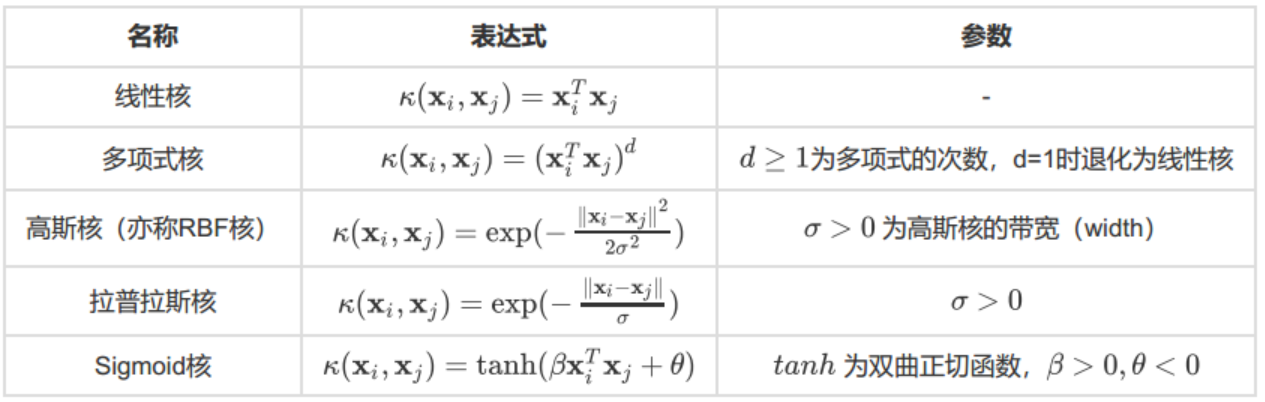
\includegraphics[scale=0.5]{04.PNG}
\end{figure}\par
特别地,文本数据一般用线性核,情况不明可尝试高斯核。除了这些常用的核函数,要产生核函数还可以使用组合的方式:\par
1.若$\kappa_1$和$\kappa_2$都是核函数,则$a\kappa_1+b\kappa_2$也是核函数,其中$a>0,b>0$。\par
2.若$\kappa_1$和$\kappa_2$都是核函数,则其直积$\kappa_1\times\kappa_2(x,z)=\kappa_1(x,z)\kappa_2(x,z)$
也是核函数。\par
3.若$\kappa_1$都是核函数,则对于任意函数$g(x)$,$\kappa(x,z)=g(x)\kappa_1(x,z)g(z)$。\newpage
\section{软间隔与正则化}
上一节中,通过利用核函数映射来解决非线性可分的问题,但现实中很难找到合适的核函数,即使某个核函数能令训练集在新特征
空间中线性可分,也难保这不是过拟合造成的结果。
\begin{figure}[ht]
    \centering
    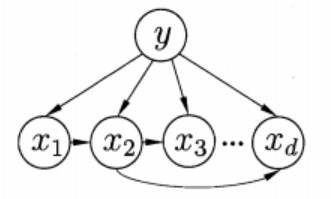
\includegraphics[scale=0.5]{05.png}
\end{figure}
比方说上面这张图,黑色虚线是此时的划分超平面,最大间隔很小。但事实上,黑色圆圈圈起的蓝点是一个outlier,可能是噪声
的原因,它偏离了正确的分布。而训练模型时,我们并没有考虑这一点,这就导致把训练样本中的outlier当成数据的真实分布拟
合了,也即过拟合。\par
但当我们允许这个outlier被误分类时,得到的划分超平面可能就如图中深红色线所示,此时的最大间隔更大,预测新样本时误分
类的概率也会降低很多。\par
在实际任务中,outlier的情况可能更加严重。比方说,如果图中的outlier再往右上移动一些距离的话,我们甚至会无法构造出一
个能将数据划分开的超平面。\par
缓解该问题的一个思路就是允许支持向量机在一些样本上出错,为此,引入软间隔(soft margin)的概念。软间隔是相对于硬间
隔(hard margin)的一个概念,硬间隔要求所有样本都必须划分正确,也即约束:
\begin{center}
    \Large{
        $y_i(\omega^Tx_i+b)\geq 1$
    }
\end{center}\par
软间隔则允许某些样本不满足约束(根据约束条件的不同,有可能某些样本出现在间隔内,甚至被误分类)。此时目标函数可以重
写为:
\begin{center}
    \Large{
        $\min\limits_{\omega,b}\frac{1}{2}||\omega||^2+C\sum\limits_{i=1}\limits^ml_{0/1}(y_i(\omega^Tx+b)-1)$\quad(12)
    }
\end{center}
其中$l_{0/1}$是0/1损失函数:
$$l_{0/1}(z)=\left\{
\begin{aligned}
    1,&if z<0\\
    0,&otherwise.
\end{aligned}    
\right.
$$\par
它的含义很简单:如果分类正确,那么函数间隔必定大于等于1,此时损失为0;如果分类错误,那么函数间隔必定小于等于-1,此
时损失为1。
而$C$则是一个大于0的常数,当$C$趋于无穷大时,式(12)等效于带约束的式(1),因为此时对误分类的惩罚无限大,也即要
求全部样本分类正确。当$C$取有限值时,允许某些样本分类错误。
由于0/1损失函数是一个非凸不连续函数,所以式(12)难以求解,于是在实际任务中,我们采用一些凸的连续函数来取替它,这
样的函数就称为替代损失(surrogate loss)函数。\par
最常用的有以下三种:
\begin{center}
    hinge损失:$l_{hinge}(z)=max(,1-z)$\\
    指数损失:$l_{exp}(z)=exp(-z)$\phantom{aaaaaaa}\\
   对率损失:$l_{log}(z)=log(1+exp(-z))$\par
\end{center}
不妨作图观察比较一下这些损失函数:
\begin{figure}[ht]
    \centering
    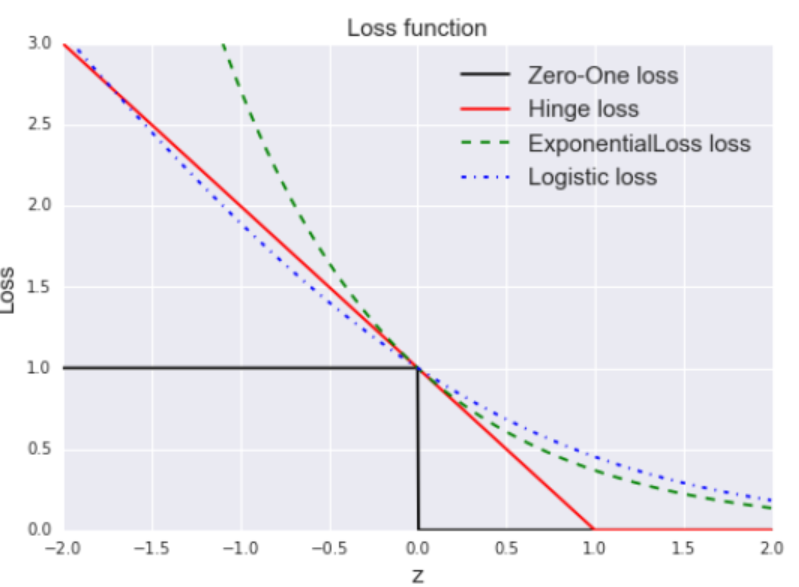
\includegraphics[scale=0.5]{06.png}
\end{figure}\\
这里有个问题是,书中提到对率损失中$log$指$ln$,也即底数为自然对数,但这种情况下对率损失在$z=0$处不为1,而是0.693。
但是书中的插图里,对率损失经过(0,1)点,此时底数应为2,上面的插图就是按底数为2计算的。实际任务中最常用的是hinge损失,
这里就以hinge损失为例,替代0/1损失函数,此时目标函数式(12)可以重写为:
\begin{center}
    \Large{
        $\min\limits_{\omega,b}\frac{1}{2}||\omega||^2+C\sum\limits_{i=1}\limits^mmax(0,1-y_i(\omega^Tx+b))$\quad(13)
    }
\end{center}
引入松弛变量(slack variables) ,可以把式(13)重写为:
\begin{center}
    \Large{
        $\min\limits_{\omega,b}\frac{1}{2}||\omega||^2+C\sum\limits_{i=1}\limits^T\xi_i$\quad(14)\\[2ex]
        $s.t.\quad y_i(w^Tx+b)\geq 1-\xi_i,\xi_i\geq 0,i=1,2,3,....,m$
    }
\end{center}
该式描述的就是软间隔支持向量机,其中每个样本都对应着一个松弛变量,用以表示该样本误分类的程度,松弛变量的值越大,程
度越高。
\subsection{软间隔支持向量机}
式(14)仍然是一个二次规划问题,我们仍用前面的方法求解:\par
1. 通过拉格朗日乘子法把$m$个约束转换$m$个拉格朗日乘子,得到该问题的拉格朗日函数。\par
2. 分别对$\omega.b,\xi$求偏导,代入拉格朗日函数得到对偶问题。\par
3. 使用SMO算法求解对偶问题,解出所有样本对应的拉格朗日乘子。\par
4. 需要进行新样本预测时,使用支持向量及其对应的拉格朗日乘子进行求解。\par
故有式(14)的拉格朗日函数:
\Large{
    \begin{align*}
        L(\omega,b,a,\xi,\mu)&=\frac{1}{2}||\omega||^2+C\sum\limits_{i=1}\limits^m\xi_i\\[2ex]
                             &+\sum\limits_{i=1}\limits^ma_i(1-\xi_i-y_i(\omega^Tx_i+b))-\sum\limits_{i=1}\limits^m\mu_i\xi_i\quad (15)
    \end{align*}
}\\
其中$a_i\geq 0,\mu_i\geq 0$是拉格朗日乘子。\par
令$L(\omega,b,a,\xi,\mu)$对$\omega,b,\xi_i$的偏导为0,可得:\par
\begin{align*}
    \omega &= \sum\limits_{i=1}\limits^ma_iy_ix_i\\[2ex]
         0 &= \sum\limits_{i=1}\limits^ma_iy_i\\[2ex]
         C &= a_i + \mu_i
\end{align*}
将上述三式代入式(15)可得式(14)的对偶问题:
\begin{center}
    \Large{
        $\max\limits_a\sum\limits_{i=1}\limits^ma_i-\frac{1}{2}\sum\limits_{i=1}\limits^m\sum\limits_{j=1}\limits^ma_ia_jy_iy_jx_i^Tx_j$ \quad (16)\\
        $s.t.\quad \sum\limits_{i=1}\limits^ma_iy_i=0,0\leq a_i\leq C,i=1,2,3,....,m$
    }
\end{center}
除去约束条件外,我们可以看出,软间隔支持向量机的对偶问题式(16)和硬间隔支持向量机的对偶问题式(5)几乎完全一致。同样的,
由于式(14)的约束条件是不等式约束,所以求解过程要求满足KKT条件:
\Large{
    $$\left\{
    \begin{aligned}
        a_i&\geq 0\\
        \mu_i&\geq 0\\
        y_i&f(x_i)-1+\xi_i\geq 0\\
        a_i&(y_if(x_i)-1+\xi_i)=0\\
        \xi_i&\geq 0\\
        \mu_i&\xi_i\geq 0
    \end{aligned}    
    \right.$$
}\par
KKT条件可以理解为:\par
1.对任意训练样本,要么对应的拉格朗日乘子$a_i=0$;要么函数间隔等于1和对应的松弛变量之差$(y_i(\omega^Tx+b)=1-\xi_i)$。\par
2.如果一个样本的拉格朗日乘子$a_i=0$,则它对模型没有任何影响,不需要保留。\par
3.如果一个样本的拉格朗日乘子大于0,则它是支持向量;若拉格朗日乘子$a_i$又小于$C$,按照式(15)有$\mu_i>0$,因此松弛变量$\xi_i=0$,
此时函数间隔为1,样本落在最大间隔边界上。若拉格朗日乘子$a_i$等于$C$,按照式(15)有$\mu_i=0$,因此松弛变量$\xi_i>0$。若
$\xi_i<1$,则样本落在间隔内,但依然被正确分类。若$\xi_i>1$,则样本落在另一个类的间隔外,被错误分类。\par
下图就展示了一个典型的软间隔支持向量机。图中就有一些异常点,这些点有的虽然在虚线与超平面之间($0<y_i(\omega^T+b)<1$),但也能
被正确分类($x_3$)。有的点落到了超平面的另一侧,就会被误分类$(x_4,x_5)$。特别地,在R.Collobert.的论文Large Scale Machine Learning
中提到,常数$C$一般取训练集大小的倒数$(\frac{1}{m})$。
\begin{figure}[ht]
    \centering
    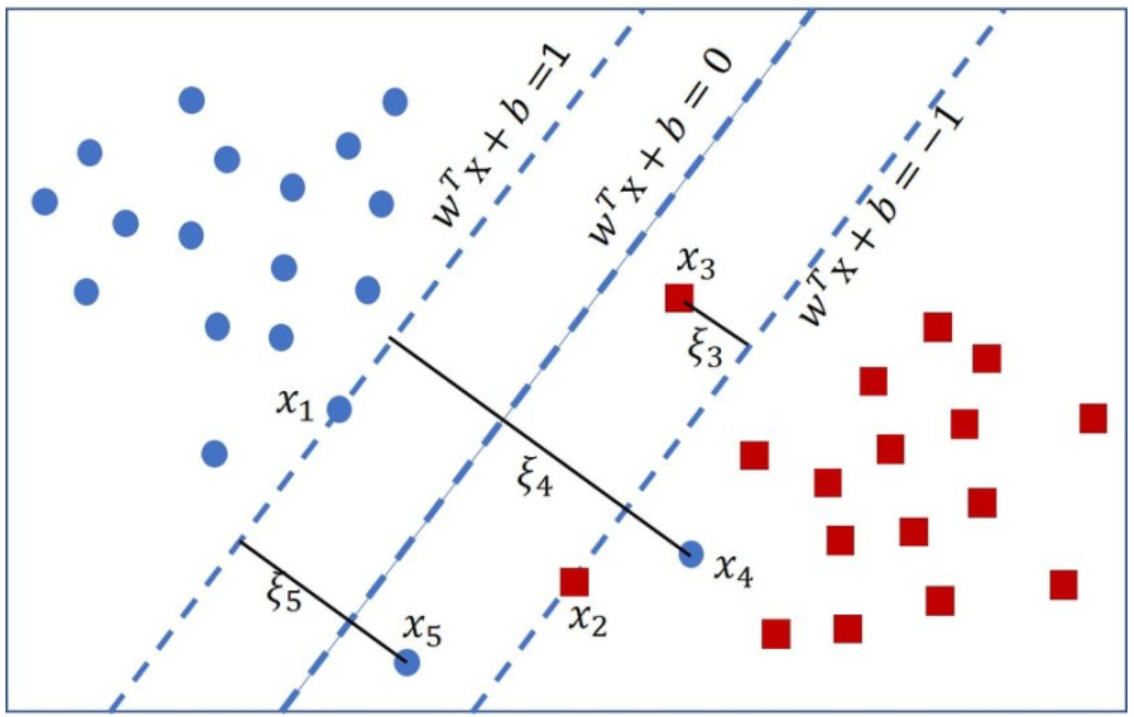
\includegraphics[scale=0.5]{07.PNG}
    \caption{软间隔支持向量机}
\end{figure}
\subsection{支持向量机和逻辑回归的联系与区别}
上面用的是hinge损失,不过我们也提到了还有其他一些替代损失函数,事实上,使用对率损失时,SVM得到的模型和LR是非常类似的。\par
支持向量机和逻辑回归的相同点:\par
1.都是线性分类器,模型求解出一个划分超平面;\par
2.两种方法都可以增加不同的正则化项;\par
3.通常来说性能相当。\par
支持向量机和逻辑回归的不同点:\par
1.LR使用对率损失,SVM一般用hinge损失;\par
2.在LR的模型求解过程中,每个训练样本都对划分超平面有影响,影响力随着与超平面的距离增大而减小,所以说LR的解受训练数据本身的分
布影响;SVM的模型只与占训练数据少部分的支持向量有关,所以说,SVM不直接依赖数据分布,所得的划分超平面不受某一类点的影响;\par
3.如果数据类别不平衡比较严重,LR需要先做相应处理再训练,SVM则不用;\par
4.SVM依赖于数据表达的距离测度,需要先把数据标准化,LR则不用(但实际任务中可能会为了方便选择优化过程的初始值而进行标准化)。如
果数据的距离测度不明确(特别是高维数据),那么最大间隔可能就变得没有意义;\par
5.LR的输出有概率意义,SVM的输出则没有;\par
6.LR可以直接用于多分类任务,SVM则需要进行扩展;\par
7.LR使用的对率损失是光滑的单调递减函数,无法导出支持向量,解依赖于所有样本,因此预测开销较大;SVM使用的hinge损
失有“零区域”,因此解具有稀疏性(书中没有具体说明这句话的意思,但按我的理解是解出的拉格朗日乘子$a$具有稀疏性,而
不是权重向量$\omega$),从而不需用到所有训练样本。\par
在实际运用中,LR更常用于大规模数据集,速度较快;SVM适用于规模小,维度高的数据集。\par
在 Andrew NG 的课里讲到过:\par
1. 如果Feature的数量很大,跟样本数量差不多,这时候选用LR或者是Linear Kernel的SVM;\par
2. 如果Feature的数量比较小,样本数量一般,不算大也不算小,选用SVM+Gaussian Kernel;\par
3. 如果Feature的数量比较小,而样本数量很多,需要手工添加一些feature变成第一种情况。\par
\subsection{正则化}
事实上,无论使用何种损失函数,SVM的目标函数都可以描述为以下形式:\par
\begin{center}
    $\min\limits_f\Omega(f)+C\sum\limits_{i=1}\limits^ml(f(x_i),y_i)$\quad (17)
\end{center}
在SVM中第一项用于描述划分超平面的“间隔”的大小,第二项用于描述在训练集上的误差。\par
更一般地,第一项称为结构风险(structural risk),用来描述模型的性质。第二项称为经验风险(empirical risk),用来描述模
型与训练数据的契合程度。参数$C$用于权衡这两种风险。\par
前面学习的模型大多都是在最小化经验风险的基础上,再考虑结构风险(避免过拟合)。SVM却是从最小化结构风险来展开的。从最
小化经验风险的角度来看, 表述了我们希望得到具有何种性质的模型(例如复杂度较小的模型),为引入领域知识和用户意图提供了
路径(比方说贝叶斯估计中的先验概率)。\par
另一方面,$\Omega(f)$还可以帮我们削减假设空间,从而降低模型过拟合的风险。从这个角度来看,可以称$\Omega(f)$为正则化
(regularization)项,$C$为正则化常数。正则化可以看作一种罚函数法,即对不希望出现的结果施以惩罚,从而使优化过程趋向
于期望的目标。\par
$L_p$范数是常用的正则化项,其中$L_2$范数$||\omega||^2$倾向于$\omega$的分量取值尽量稠密,即非零分量个数尽量多;$L_0$
范$||\omega||_0$和范数$||\omega||_1$则倾向于$\omega$的分量取值尽量稀疏,即非零分量个数尽量少。\newpage
\section{支持向量回归}
同样是利用线性模型$f(x)=\omega^Tx+b$来预测,回归问题希望预测值和真实值$y$尽可能相近,而不是像分类任务那样,旨在令不
同类的预测值可以被划分开。\par
传统的回归模型计算损失时直接取真实值和预测值的差,支持向量回归(Support Vector Regression,简称SVR)则不然。SVR
假设我们能容忍最多有$\epsilon$的偏差,只有当真实值和预测值之间相差超出了$\epsilon$时才计算损失。\par
\begin{figure}[ht]
    \centering
    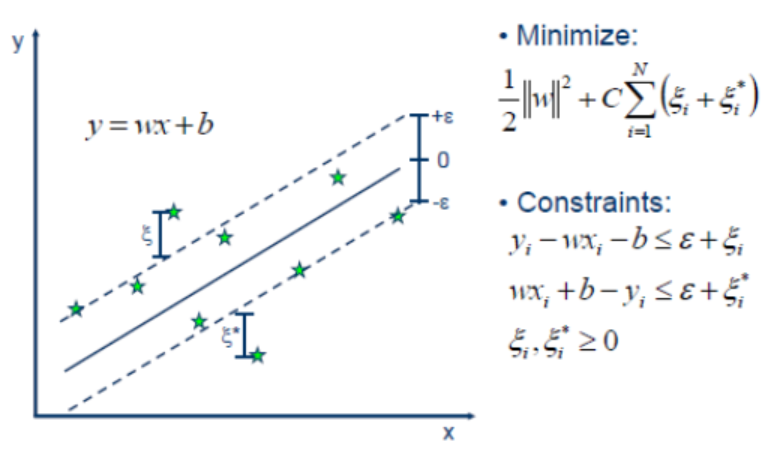
\includegraphics[scale=0.5]{08.PNG}    
\end{figure}\par
如图所示,以SVR拟合出的直线为中心,两边各构建出一个宽度为$\epsilon$的地带,落在这个宽度为$2\epsilon$的间隔带内的点
都被认为是预测正确的。\par
因此,问题可以形式化为目标函数:\par
\begin{center}
    \Large{
        $\min\limits_{\omega,b}\frac{1}{2}||\omega||^2+C\sum\limits_{i=1}\limits^ml_{\epsilon}(f(x_i)-y_i)$
    }
\end{center}
其中$C$为正则化常数,$l_{\epsilon}$称为$\epsilon-$不敏感损失(insensitive loss)函数。定义如下:
$$l_{\epsilon}(z)=\left\{
    \begin{aligned}
    &0,if|z|<0;\\
    &|z|-\epsilon,otherwise\\
    \end{aligned}
\right.
$$
引入松弛变量$\xi_i$
和$\xi_j$,分别表示间隔带两侧的松弛程度,它们可以设定为不同的值。此时,目标函数式(18)可以重写为:
\begin{center}
    \Large{
        $\min\limits_{\omega,b}\frac{1}{2}||\omega||^2+C\sum\limits_{i=1}\limits^m(\xi_i+\hat{\xi_i})$\quad(19)\\[2ex]
        $s.t. f(x_i)-y_i\leq \epsilon+\xi_i,y_i-f(x_i)\leq \epsilon+\xi_i,\xi_i\geq 0,$\\[2ex]
        $\hat{\xi_i}\geq 0,i=1,2,...,m$
    }
\end{center}
注意这里有四组$m$个约束条件,所以对应地有四组拉格朗日乘子。\par
接下来就是用拉格朗日乘子法获得问题对应的拉格朗日函数,然后求偏导再代回拉格朗日函数,得到对偶问题。然后使用SMO算
法求解拉格朗日乘子,最后得到模型,这里不一一详述了。\par
特别地,SVR中同样有支持向量的概念,解具有稀疏性,所以训练好模型后不需保留所有训练样本。此外,SVR同样可以通过引入
核函数来获得拟合非线性分布数据的能力。\newpage
\section{核方法}
给定训练样本${(x_1,y_1),(x_2,y_2),...,(x_m,y_m)}$,若不考虑偏移项b,无论是$SVM$还是$SVR$,模型总可以表示为核函数
$\kappa(x,x_i)$的线性组合。不仅如此,我们有定理:\par
令$\mathbb{H}$为核函数$\kappa$的再生希尔伯特空间,$||h||_\mathbb{H}$表示$\mathbb{H}$空间中关于h的范数,对于任意
单调递增函数$\Omega:[0,\infty]\to \mathbb{R}$和任意非负损失的函数$l:\mathbb{R}^m\to [0,\infty]$,优化问题:
\begin{center}
    $\min_{h\in\mathbb{H}}F(h)=\Omega(||h||_{\mathbb{H}})+l(h(x_1,h(x_2,...,h(x_m))))$\quad(20)
\end{center}
的解总可以写为:\par
\begin{center}
    $h^x(x)=\sum\limits_{i=1}\limits^ma_i\kappa(x,x_i)$
\end{center}
这个定理表明,对于形如式(20),旨在最小化损失和正则化项之和的优化问题,解都可以表示为核函数的线性组合。基于核函数的
学习方法,统称为核方法(kernal methods)。最常见的就是通过核化(引入核函数),将线性学习器扩展为非线性学习器。这不仅
限于SVM,事实上LR和LDA也都可以采用核函数,只是SVM使用hinge损失,解具有稀疏性所以用得更多。
}
\end{document}

